\documentclass[border=3pt]{standalone}
% Shared preamble for standalone figures (same fonts/colours as the paper).
\usepackage[T1]{fontenc}
\usepackage{lmodern}
\usepackage{amsmath,amssymb}
\usepackage[dvipsnames,svgnames]{xcolor}
\usepackage{tikz}
\usetikzlibrary{arrows.meta,positioning,calc,shapes.geometric,decorations.pathreplacing,shadings}
\usepackage{pgfplots}
\pgfplotsset{compat=1.18}
\usepgfplotslibrary{fillbetween}
\definecolor{pgrey}{HTML}{EEEEEE}
\definecolor{ppink}{HTML}{F8D7DA}
\definecolor{ppeach}{HTML}{FDE5C8}
\definecolor{porange}{HTML}{FBC78D}
\definecolor{pgreen}{HTML}{D4F7D4}
\definecolor{ppurple}{HTML}{EFE3F7}
\definecolor{pblue}{HTML}{DCE8F7}
\definecolor{dgreen}{HTML}{2E8B2E}
\definecolor{dpink}{HTML}{C2185B}
\definecolor{dorange}{HTML}{E07B00}
\definecolor{dblue}{HTML}{1F4E9E}
\definecolor{dpurple}{HTML}{7B3FA0}
\definecolor{gold}{HTML}{E0A800}
\tikzset{
  blk/.style={draw=black!70,rounded corners=2pt,minimum height=0.8cm,minimum width=1.9cm,
              align=center,font=\sffamily\footnotesize,inner sep=3pt},
  arr/.style={-{Stealth[length=2.2mm]},thick,black!75},
  darr/.style={-{Stealth[length=2mm]},dashed,thick},
  lbl/.style={font=\itshape\scriptsize},
}

\begin{document}
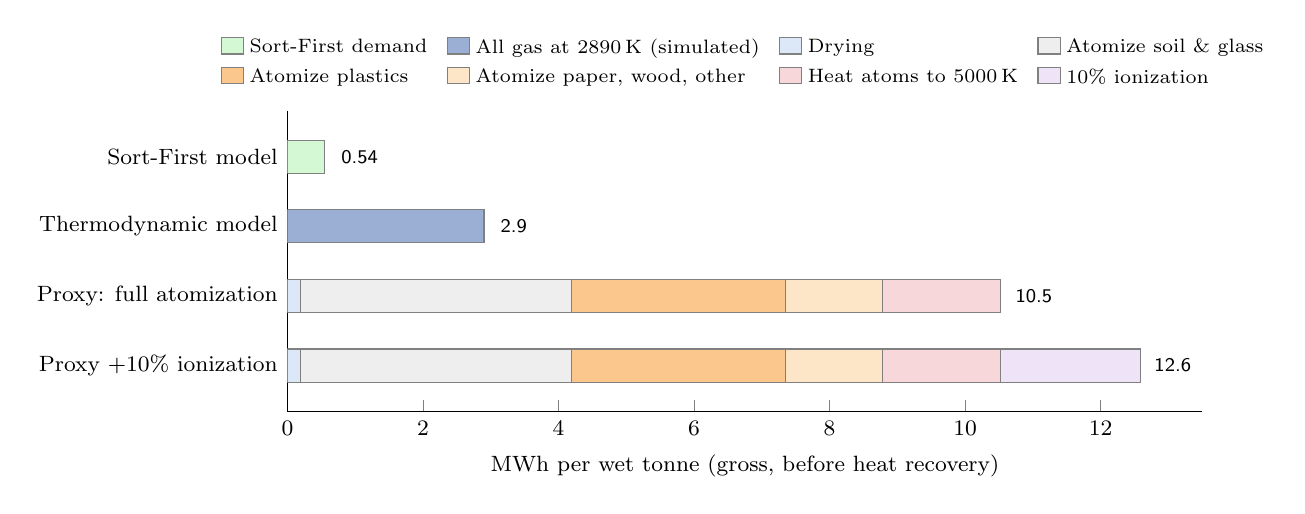
\begin{tikzpicture}
\begin{axis}[xbar stacked, width=13.2cm, height=5.4cm, bar width=0.42cm, xmin=0, xmax=13.5,
  ytick=data, yticklabels={{Sort-First model},{Thermodynamic model},{Proxy: full atomization},{Proxy +10\% ionization}},
  y dir=reverse, xlabel={MWh per wet tonne (gross, before heat recovery)},
  legend style={at={(0.5,1.04)},anchor=south,legend columns=4,font=\scriptsize,draw=none,
    /tikz/every even column/.append style={column sep=5pt}},
  legend cell align=left, tick label style={font=\footnotesize}, label style={font=\footnotesize},
  enlarge y limits=0.22, axis x line*=bottom, axis y line*=left]
\addplot[fill=pgreen,draw=black!50] coordinates {(0.543,0) (0,1) (0,2) (0,3)}; \addlegendentry{Sort-First demand}
\addplot[fill=dblue!45,draw=black!50] coordinates {(0,0) (2.90,1) (0,2) (0,3)}; \addlegendentry{All gas at 2890\,K (simulated)}
\addplot[fill=pblue,draw=black!50] coordinates {(0,0) (0,1) (0.196,2) (0.196,3)}; \addlegendentry{Drying}
\addplot[fill=pgrey,draw=black!50] coordinates {(0,0) (0,1) (3.997,2) (3.997,3)}; \addlegendentry{Atomize soil \& glass}
\addplot[fill=porange,draw=black!50] coordinates {(0,0) (0,1) (3.156,2) (3.156,3)}; \addlegendentry{Atomize plastics}
\addplot[fill=ppeach,draw=black!50] coordinates {(0,0) (0,1) (1.427,2) (1.427,3)}; \addlegendentry{Atomize paper, wood, other}
\addplot[fill=ppink,draw=black!50] coordinates {(0,0) (0,1) (1.748,2) (1.748,3)}; \addlegendentry{Heat atoms to 5000\,K}
\addplot[fill=ppurple,draw=black!50] coordinates {(0,0) (0,1) (0,2) (2.07,3)}; \addlegendentry{10\% ionization}
\node[font=\sffamily\scriptsize,anchor=west] at (axis cs:0.65,0) {0.54};
\node[font=\sffamily\scriptsize,anchor=west] at (axis cs:3.0,1) {2.9};
\node[font=\sffamily\scriptsize,anchor=west] at (axis cs:10.6,2) {10.5};
\node[font=\sffamily\scriptsize,anchor=west] at (axis cs:12.65,3) {12.6};
\end{axis}
\end{tikzpicture}
\end{document}
